\documentclass[12pt]{article}

\usepackage{discrete}

\def\thetitle{Functions} % will be put in the center header on the first page only.
\def\lefthead{Math 228 Notes} % will be put in the left header
\def\righthead{Functions} % will be put in the right header


\begin{document}

A function\index{function} is a rule that assigns each input exactly one output.  The set of all inputs for a function is called the \emph{domain}\index{domain}.  The set of all allowable outputs is called the \emph{codomain}\index{codomain}.  For example, a function might assign each natural number a natural number from 1 to 5.  In that case, the domain is the natural numbers and the codomain is the set of natural numbers from 1 to 5. Now it could be that this particular function we are thinking about assigns each even natural number to the number 2 and each odd natural number to the number 1.  In this case, not all of the codomain is actually used.  We would say that the set $\{1,2\}$ is the \emph{range}\index{range} of the function. These are the elements in the codomain (allowable outputs) which are actually outputs for some input. 

The key thing that makes a rule assigning inputs to outputs a \emph{function} is that there is \emph{only one} output for an input.  In other words, it is important that the rule be a good rule.  What output do we assign to the input 7?  There can only be one answer for any particular function. 

To specify the name of the function, as well as the domain and codomain, we write $f:X \to Y$.  The function is called $f$, the domain is the set $X$ and the codomain is the set $Y$.  This however does not describe the rule.  To do that, we say something like this:

\begin{quote}
  The function $f:X \to Y$ is defined by $f(x) = x^2 + 3$.
\end{quote}

This function takes an input $x$ and computes the output by squaring $x$ and then adding 3.  In this case, you better hope that $X$ is a set of numbers and $Y$ is a set of number which can be 3 more than squares of numbers from $X$.  It would not work for $Y$ to be negative numbers here. That would not be a valid function.

The description of the rule can vary greatly.  If $X$ is a finite set, we might just give a list of each output for each input.  You could also describe the function with a table or a graph or in words.

\begin{example}
  The following are all examples of functions:
  \begin{enumerate}
    \item $f:\Z \to \Z$ defined by $f(n) = 3n$.  The domain and codomain are both the set of integers.  However, the range is only the set of integer multiples of 3.
    \item $f: \{1,2,3\} \to \{a,b,c\}$ defined by $f(1) = c$, $f(2) = a$ and $f(3) = a$.  The domain is the set $\{1,2,3\}$, the codomain is the set $\{a,b,c\}$ and the range is the set $\{a,c\}$.  Note that $f(2)$ and $f(3)$ are the same element of codomain.  This is not a problem.  Each element in the domain still has only one output (although each output does not have a unique input).
    \item $f:\{1,2,3\} \to \{1,2,3\}$ defined as follows:
    \begin{center}
      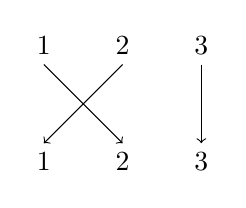
\begin{tikzpicture}
        \draw[->] (-1,1) node[above] {1} -- (0,0) node[below] {2};
        \draw[->] (0,1) node[above] {2} -- (-1,0) node[below] {1};
        \draw[->] (1,1) node[above] {3} -- (1,0) node[below] {3};
      \end{tikzpicture}

    \end{center}

  \end{enumerate}

\end{example}

The arrow diagram used to define the function above can be very helpful in visualizing functions.  We will often be working with functions on finite sets so this kind of picture is often more useful than a traditional graph of a function.  A graph of the function in example 3 above would look like this:

\begin{center}
  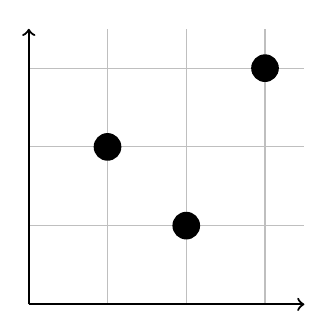
\begin{tikzpicture}
    %axis:
    \draw[thin, gray!50] (0,0) grid (3.5, 3.5);
    \draw[->, thick] (0,0) -- (0,3.5);
   \draw[->, thick] (0,0) -- (3.5,0);
   %points:
   \fill (1,2) circle (5pt) (2,1) circle (5pt) (3,3) circle (5pt);
  \end{tikzpicture}

\end{center}

It would be absolutely WRONG to connect the dots or try to fit them to some curve.  There are only three elements in the domain.  A curve suggests that the domain contains an entire interval of real numbers.  Remember, we are not in calculus any more!

It is important to know how to recognize a function from a rule which is not a function.  The arrow diagram can help.

\begin{example}
Which of the following diagrams represent a function.  Let $X = \{1,2,3,4\}$ and $Y = \{a,b,c,d\}$
  \begin{multicols}{3}
    \begin{center}
      $f:X \to Y$
      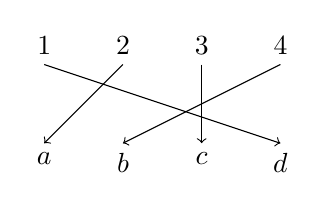
\begin{tikzpicture}
        \draw[->] (-1.5,1) node[above] {1} -- (1.5,0) node[below] {$d$};
        \draw[->] (-.5,1) node[above] {2} -- (-1.5,0) node[below] {$a$};
        \draw[->] (.5,1) node[above] {3} -- (.5, 0) node[below] {$c$};
        \draw[->] (1.5,1) node[above] {4} -- (-.5, 0) node[below] {$b$};
      \end{tikzpicture}
      \columnbreak
      
      $g:X \to Y$
	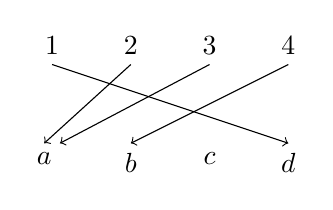
\begin{tikzpicture}
        \draw[->] (-1.5,1) node[above] {1} -- (1.5,0) node[below] {$d$};
        \draw[->] (-.5,1) node[above] {2} -- (-1.6,0) node[below] {$a$};
        \draw[->] (.5,1) node[above] {3} -- (-1.4, 0);
        \draw[->] (1.5,1) node[above] {4} -- (-.5, 0) node[below] {$b$};
        \draw (.5,0) node[below] {$c$};
      \end{tikzpicture}
      
      \columnbreak
      
      $h:X \to Y$
      	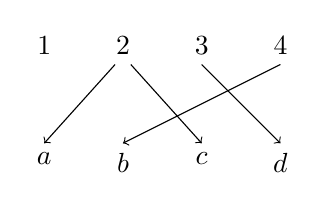
\begin{tikzpicture}
        \draw (-1.5,1) node[above] {1};
        \draw[->] (-.5,1) node[above] {2} (-.6,1) -- (-1.5,0) node[below] {$a$};
        \draw[->] (-.4,1) -- (.5,0);
        \draw[->] (.5,1) node[above] {3} -- (1.5, 0) node[below] {$d$};
        \draw[->] (1.5,1) node[above] {4} -- (-.5, 0) node[below] {$b$};
        \draw (.5,0) node[below] {$c$};
      \end{tikzpicture}
    \end{center}

  \end{multicols}
\begin{solution}
  $f$ is a function.  So is $g$.  There is no problem with an element of the codomain not being the output for any input, and there is no problem with $a$ from the codomain being the output of both 2 and 3 from the domain.  
  
  However, $h$ is \textbf{not} a function.  In fact, it fails for two reasons.  First, the element 1 from the domain has not been mapped to any element from the codomain.  Second, the element 2 from the domain has been mapped to more than one element from the codomain ($a$ and $c$).  Note that either one of these problems is enough to make a rule not a function.  Neither of these mappings are functions:
  \begin{center}
    \begin{multicols}{2}
      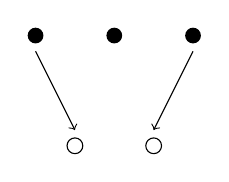
\begin{tikzpicture}
        \fill (-1, 1.2) circle (.1) (0,1.2) circle (.1) (1, 1.2) circle (.1);
        \draw[->] (-1, 1) -- (-.5,0);
        \draw[->] (1,1) -- (.5, 0);
        \draw (-.5, -0.2) circle (.1) (.5, -0.2) circle (.1);
      \end{tikzpicture}
       
       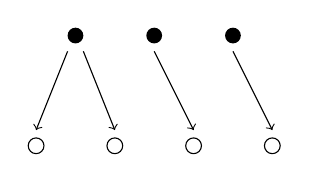
\begin{tikzpicture}
         \fill (-1, 1.2) circle (.1) (0,1.2) circle (.1) (1, 1.2) circle (.1);
         \draw[->] (-1.1, 1) -- (-1.5, 0);
         \draw[->] (-.9, 1) -- (-.5, 0);
         \draw[->] (0,1) -- (.5,0);
         \draw[->] (1,1) -- (1.5, 0);
         \draw (-.5, -0.2) circle (.1) (.5, -0.2) circle (.1) (-1.5, -0.2) circle (.1) (1.5, -0.2) circle (.1);
       \end{tikzpicture}

    \end{multicols}
  Not functions.
  \end{center}

\end{solution}

\end{example}

\subsection{Surjections, Injections, and Bijections}

We now turn to investigating special properties functions might or might not possess.  

In the examples above, you may have noticed that sometimes there are elements of the codomain which are not in the range.  When this sort of the thing \emph{does not} happen, (that is, when everything in the codomain is in the range) we say the function is \emph{onto}\index{onto|see {surjection}} or that the function maps the domain \emph{onto} the codomain.  This terminology should make sense: the function puts the domain (entirely) on top the codomain.  The fancy math term for an onto function is a \emph{surjection}\index{surjection}, and we say that an onto function is a \emph{surjective} function.

In pictures:

\begin{multicols}{2}
  \begin{center}
          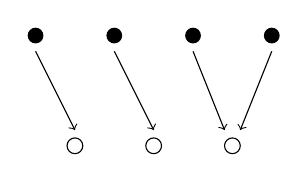
\begin{tikzpicture}
        \fill (-1.5, 1.2) circle (.1) (-.5,1.2) circle (.1) (.5, 1.2) circle (.1) (1.5,1.2) circle (.1);
        \draw[->] (-1.5, 1) -- (-1,0);
        \draw[->] (-.5,1) -- (0, 0);
        \draw[->] (.5, 1) -- (.9,0);
        \draw[->] (1.5,1) -- (1.1,0);
        \draw (-1, -0.2) circle (.1) (0, -0.2) circle (.1) (1, -0.2) circle (.1);
      \end{tikzpicture}
      
      Surjective
      
      \columnbreak
      
                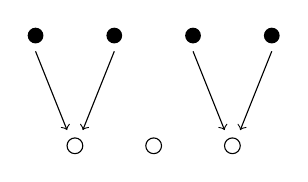
\begin{tikzpicture}
        \fill (-1.5, 1.2) circle (.1) (-.5,1.2) circle (.1) (.5, 1.2) circle (.1) (1.5,1.2) circle (.1);
        \draw[->] (-1.5, 1) -- (-1.1,0);
        \draw[->] (-.5,1) -- (-.9, 0);
        \draw[->] (.5, 1) -- (.9,0);
        \draw[->] (1.5,1) -- (1.1,0);
        \draw (-1, -0.2) circle (.1) (0, -0.2) circle (.1) (1, -0.2) circle (.1);
      \end{tikzpicture}
      
      Not surjective
  \end{center}

\end{multicols}

\begin{example}
  Which functions are surjective (i.e., onto)?
    \begin{enumerate}
    \item $f:\Z \to \Z$ defined by $f(n) = 3n$.  
    \item $g: \{1,2,3\} \to \{a,b,c\}$ defined by $g(1) = c$, $g(2) = a$ and $g(3) = a$.  
    \item $h:\{1,2,3\} \to \{1,2,3\}$ defined as follows:
    \begin{center}
      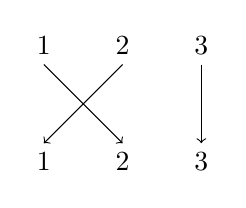
\begin{tikzpicture}
        \draw[->] (-1,1) node[above] {1} -- (0,0) node[below] {2};
        \draw[->] (0,1) node[above] {2} -- (-1,0) node[below] {1};
        \draw[->] (1,1) node[above] {3} -- (1,0) node[below] {3};
      \end{tikzpicture}
    \end{center}
  \end{enumerate}
  \begin{solution}
    \begin{enumerate}
      \item $f$ is not surjective.  There are elements in the codomain which are not in the range.  For example, no $n \in \Z$ gets mapped to the number 1 (the rule would say that $\frac{1}{3}$ would be sent to 1, but $\frac{1}{3}$ is not in the domain).  In fact, the range of the function is $3\Z$ (the integer multiples of 3), which is not equal to $\Z$.
      \item $g$ is not surjective.  There is no $x \in \{1,2,3\}$ (the domain) for which $g(x) = b$.  So $b$, which is in the codomain, is not in the range, so once again the function is not onto.
      \item $h$ is surjective.  Every element of the codomain is also in the range.  Nothing is missed.
    \end{enumerate}

  \end{solution}

\end{example}


To be a function, a map cannot assign a single element of the domain to two or more different elements of the codomain.  However, we have seen that the reverse is permissible.  That is, a function might assign the same element of the codomain to two or more different elements of the domain.  When this \emph{does not} occur (that is, when each element of the codomain is assigned to at most one element of the domain) then we say the function is \emph{one-to-one}\index{one-to-one|see {injection}}.  Again, this terminology makes sense: we are sending at most one element from the domain to one element from the codomain.  One input to one output. The fancy math term for a one-to-one function is an \emph{injection}\index{injection}.  We call one-to-one functions \emph{injective} functions.

In pictures:

\begin{multicols}{2}
  \begin{center}
          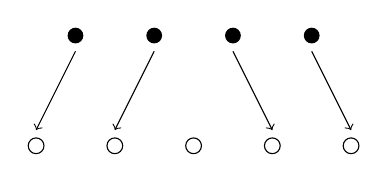
\begin{tikzpicture}
        \fill (-1.5, 1.2) circle (.1) (-.5,1.2) circle (.1) (.5, 1.2) circle (.1) (1.5,1.2) circle (.1);
        \draw[->] (-1.5, 1) -- (-2,0);
        \draw[->] (-.5,1) -- (-1, 0);
        \draw[->] (.5, 1) -- (1,0);
        \draw[->] (1.5,1) -- (2,0);
        \draw (-2, -0.2) circle (.1) (-1, -.2) circle (.1) (0, -0.2) circle (.1) (1, -0.2) circle (.1) (2, -0.2) circle (.1);
      \end{tikzpicture}
      
      Injective
      
      \columnbreak
      
                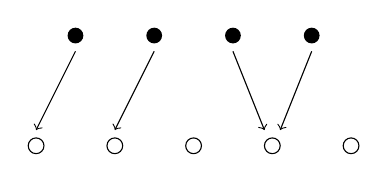
\begin{tikzpicture}
        \fill (-1.5, 1.2) circle (.1) (-.5,1.2) circle (.1) (.5, 1.2) circle (.1) (1.5,1.2) circle (.1);
        \draw[->] (-1.5, 1) -- (-2,0);
        \draw[->] (-.5,1) -- (-1, 0);
        \draw[->] (.5, 1) -- (.9,0);
        \draw[->] (1.5,1) -- (1.1,0);
        \draw (-2, -0.2) circle (.1) (-1, -.2) circle (.1) (0, -0.2) circle (.1) (1, -0.2) circle (.1) (2, -0.2) circle (.1);
      \end{tikzpicture}
      
      Not injective
  \end{center}

\end{multicols}


\begin{example}
  Which functions are injective (i.e., one-to-one)?
    \begin{enumerate}
    \item $f:\Z \to \Z$ defined by $f(n) = 3n$.  
    \item $g: \{1,2,3\} \to \{a,b,c\}$ defined by $g(1) = c$, $g(2) = a$ and $g(3) = a$.  
    \item $h:\{1,2,3\} \to \{1,2,3\}$ defined as follows:
    \begin{center}
      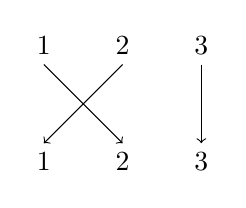
\begin{tikzpicture}
        \draw[->] (-1,1) node[above] {1} -- (0,0) node[below] {2};
        \draw[->] (0,1) node[above] {2} -- (-1,0) node[below] {1};
        \draw[->] (1,1) node[above] {3} -- (1,0) node[below] {3};
      \end{tikzpicture}
    \end{center}
  \end{enumerate}
  \begin{solution}
    \begin{enumerate}
      \item $f$ is injective.  Each element in the codomain is assigned to at \emph{most} one element from the domain.  If $x$ is a multiple of three, then only $x/3$ is mapped to $x$.  If $x$ is not a multiple of 3, then there is no input corresponding to the output $x$.
      \item $g$ is not injective.  Both inputs $2$ and $3$ are assigned the output $a$.
      \item $h$ is injective.  Each output is only an output once.
    \end{enumerate}

  \end{solution}

\end{example}



From the examples above, it should be clear that there are functions which are surjective, injective, both or neither.  In the case when a function is both one-to-one and onto (a injection and surjection) we say the function is a \emph{bijection}, or that the function is a \emph{bijective} function.  

\subsection{Inverse Image}

When discussing functions, we have notation for talking about an element of the domain (say $x$) and its corresponding element in the codomain (we write $f(x)$).  It would also be nice to start with some element of the codomain (say $y$) and talk about which element or elements (if any) from the domain get sent to it.  We could write ``those $x$ in the domain such that $f(x) = y$,'' but this is a lot of writing.  So here is some notation to make our lives easier.

Suppose $f:X \to Y$ is a function.  For $y \in Y$ (an element of the codomain), we write $f\inv(y)$ to represent the \emph{set} of all elements in the domain $X$ which get sent to $y$.  That is, $f\inv(y) = \{x \in X \st f(x) = y\}$.  We say that $f\inv(y)$ is the \emph{complete inverse image}\index{inverse image} of $y$ under $f$.

\vskip 1em
\noindent\textbf{WARNING: $f\inv(y)$ is not an inverse function!!!!  Inverse functions only exist for bijections, but $f\inv(y)$ is defined for any function $f$.  The point: $f\inv(y)$ is a \underline{set}, not an element of the domain.}
\vskip 1em

\begin{example}
 Consider the function $f:\{1,2,3,4,5,6\} \to \{a,b,c,d\}$ given by $f(1) = a$, $f(2) = a$, $f(3) = b$, $f(4) = c$, $f(5) = c$ and $f(6) = c$.  Find the complete inverse image of each element in the codomain.
 \begin{solution}
  Remember, we are looking for sets.
  \[f\inv(a) = \{1,2\}\]
  \[f\inv(b) = \{3\}\]
  \[f\inv(c) = \{4,5,6\}\]
  \[f\inv(d) = \emptyset.\]
 \end{solution}
\end{example}

\begin{example} Consider the function $g:\Z \to \Z$ defined by $g(n) = n^2 + 1$.  Find $g\inv(1)$, $g\inv(2)$, $g\inv(3)$ and $g\inv(10)$.
 \begin{solution}
  To find $g\inv(1)$, we need to find all integers $n$ such that $n^2 + 1 = 1$.  Clearly only 0 works, so $g\inv(1) = \{0\}$ (note that even though there is only one element, we still write it as a set with one element in it).  
  
  To find $g\inv(2)$, we need to find all $n$ such that $n^2 + 1 = 2$.  We see $g\inv(2) = \{-1,1\}$.  
  
  If $n^2 + 1 = 3$, then we are looking for an $n$ such that $n^2 = 2$.  There are no such integers so $g\inv(3) = \emptyset$. 
  
  Finally, $g\inv(10) = \{-3, 3\}$ because $g(-3) = 10$ and $g(3) = 10$.
 \end{solution}

\end{example}

Since $f\inv(y)$ is a set, it makes sense to ask for $|f\inv(y)|$, the number of elements in the domain which map to $y$.

\begin{example}
 Find a function $f:\{1,2,3,4,5\} \to \N$ such that $|f\inv(7)| = 5$.  
 \begin{solution}
 There is only one such function.  We need five elements of the domain to map to the number $7 \in \N$.  Since there are only five elements in the domain, all of them must map to 7.  So $f(1) = 7$, $f(2) = 7$, $f(3) = 7$, $f(4) = 7$ and $f(5) = 7$.
 \end{solution}
\end{example}





\begin{defbox}{Function Definitions}
\begin{itemize}
  \item A \emph{function} is a rule that assigns each element of a set, called the \emph{domain}, to exactly one element of a second set, called the \emph{codomain}.
  \item Notation: $f:X \to Y$ is our way of saying that the function is called $f$, the domain is the set $X$ and the codomain is the set $Y$.
  \item $f(x) = y$ means the element $x$ of the domain (input) is assigned to the element $y$ of the codomain.  We say $y$ is an output.  Alternatively, we call $y$ the \emph{image of $x$ under $f$}.
  \item The \emph{range} is a subset of the codomain.  It is the set of all elements which are assigned to at least one element of the domain by the function.  That is, the range is the set of all outputs.
  \item A function is \emph{injective} (an \emph{injection} or \emph{one-to-one}) if every element of the codomain is the output for \textbf{at most} one element from the domain.
  \item A function is \emph{surjective} (a \emph{surjection} or \emph{onto}) if every element of the codomain is the output of \textbf{at least} one element of the domain.
  \item A \emph{bijection} is a function which is both an injection and surjection.  In other words, if every element of the codomain is the output of \textbf{exactly one} element of the domain.
  \item The \emph{complete inverse image} of an element in the codomain, written $f\inv(y)$ is the \textbf{set} of all element in the domain which are assigned to $y$ by the function.  
\end{itemize}

\end{defbox}



\end{document}
